% This is "sig-alternate.tex" V2.0 May 2012
% This file should be compiled with V2.5 of "sig-alternate.cls" May 2012
%
% For tracking purposes - this is V2.0 - May 2012

\documentclass[letterpaper]{www13-companion-accepted}
% \pdfpagewidth=8.5in
% \pdfpageheight=11in
% \usepackage[paperwidth=8.5in,paperheight=11in]{geometry}
\special{papersize=8.5in,11in}
\usepackage{graphicx}
\usepackage{subfigure}
\usepackage{url}
% \usepackage{indentfirst}
\usepackage{cite}
\usepackage[T1]{fontenc}
\usepackage{color}
\newcommand{\red}[1]{\textcolor{red}{#1}}
\newcommand{\blue}[1]{\textcolor{blue}{#1}}

%\usepackage[normalem]{ulem}

\def\sharedaffiliation{%
\end{tabular}
\begin{tabular}{c}}

\begin{document}
%
% --- Author Metadata here ---
\conferenceinfo{WWW 2013 Companion}{May 13-17, 2013, Rio de Janeiro, Brazil.}
%\CopyrightYear{2007} % Allows default copyright year (20XX) to be over-ridden - IF NEED BE.
%\crdata{0-12345-67-8/90/01}  % Allows default copyright data (0-89791-88-6/97/05) to be over-ridden - IF NEED BE.
% --- End of Author Metadata ---

%\title{Temporal Evolution of Scientific Communities}
\title{The Role of Research Leaders on the \\ Evolution of Scientific Communities}
%\title{The Role of Leaders in the Dynamics of Scientific Communities}


\numberofauthors{3} %  in this sample file, there are a *total*
%
% 1st. author
%\alignauthor Bruno Leite Alves, Fabr\'icio Benevenuto, Alberto H. F. Laender\\
%       \affaddr{Departamento de Ci\^encia da Computa\c{c}\~ao}\\
%       \affaddr{Universidade Federal de Minas Gerais}\\
%       \affaddr{Belo Horizonte, Brazil}\\
%       \email{\{bruno.leite,Fabricio,Laender\}@dcc.ufmg.br}


\author{
\alignauthor Bruno Leite Alves\\
\alignauthor Fabr\'icio Benevenuto\\
\alignauthor Alberto H. F. Laender
\and
\sharedaffiliation
\affaddr{Departamento de Ci\^encia da Computa\c{c}\~ao}\\
\affaddr{Universidade Federal de Minas Gerais}\\
\affaddr{Belo Horizonte, MG, Brazil}\\
\affaddr{\{bruno.leite, fabricio, laender\}@dcc.ufmg.br}
}


\maketitle
\begin{abstract}

\noindent
There have been considerable efforts in the literature towards understanding and modeling dynamic aspects of 
scientific communities. Despite the great interest, little is known about the role that different members play 
in the formation of the underlying network structure of such communities. In this paper, we provide a wide 
investigation of the roles that members of the core of scientific communities play in the collaboration network 
structure formation and evolution. To do that, we define a community core based on an individual metric, 
\textit{core score}, which is an h-index derived metric that captures both, the prolificness and the involvement
of researchers in a community. Our results provide a number of key observations related to community formation and 
evolving patterns. Particularly, we show that members of the community core work as bridges that connect smaller 
clustered research groups. Furthermore, these members are responsible for an increase in 
the average degree of the whole community underlying network and a decrease on the overall network assortativeness. 
More important, we note that variations on the members of the community core tend to be strongly correlated with 
variations on these metrics. We argue that our observations are important for shedding a light on the role of key 
members on community formation and structure.
\end{abstract}

% \vspace{-0.1cm}
\category{J.4.} {Computer Applications} Social and Behavioral Sciences
% \vspace{0.15cm}
\terms{Human Factors, Measurement.}
% \vspace{0.15cm}
\keywords{Scientific Communities, Core Community, Community Evolution.}
\vspace{1.4cm}
% \\ \\ \\ \\
\section{Introduction}

Since its beginning, society has been organizing itself into communities, which are groups of individuals with common interests\footnote{http://www.merriam-webster.com/dictionary/community}.
Particularly, the proliferation of new communication technologies based on the Internet has facilitated the rapid formation and growth of online communities~\cite{Kleinberg@cacm2008}. 
Communities exhibit a wide range of characteristics and serve a variety of purposes, from small groups engaged in tightly niche topics such as a very specific scientific community, 
to millions of users linked by an interest such as a community related to a sport team or fans of a celebrity. 

Often, individuals who are socially connected in a tend to share interests and similarities. Although, there are many factors that might determine a community formation
and its growth, there are two main driven forces used to explain similarity in a community formation: influence and homophily. On one hand, influence posits that individuals change
to become more similar to their friends in the community. On the other hand, homophily postulates that individuals create social connections within a community precisely because
they are already similar. Recent efforts have provided quantitative evidences of both forces~\cite{icwsm10cha,crandall.kdd08,Backstrom:2006,influence.correlation.kdd08} and
existing theories~\cite{Rogers.1962,accidental-influential}, models~\cite{kempe03kdd,Kempe05influentialnodes}, and
approaches~\cite{saez-trumper@kdd12,Weng:2010:TFT:1718487.1718520} rely on identifying a group of influential individuals with the power to affect not only the underlying network
structure of a community, but also to interfere on the spread and flow of information within a community. 

In this paper, we take a different perspective and study a complementary problem. Here, we focus on studying the roles that influential individuals from a scientific community play
on evolving properties of such communities. Intuitively, when prolific research leaders decide to join or leave a community, they take with them resources,
experience and students, and they possibly influence other members to do the same, which makes scientific communities very suitable for this kind of study. To construct these
communities we used data from DBLP to identify scientific communities, represented by the main ACM SIG conferences. Then, we propose a strategy to infer the community core, 
the leaders of a given scientific community in a given period of time. Finally, we investigate how aspects of the core impact on the community underlying structure. 

The study of the core of scientific communities is of interest from two different perspectives.  The first is sociological, coming from the necessity to understand how
segments of society evolve as well as to answer longstanding  questions related to the interaction among different types of participant. On the other hand, from a technological perspective,
understanding these aspects is critical not only for link prediction, but also for the design of better recommendation systems. 
Such a study, however, has been difficult as essential components like human connections and a proper definition of leadership is hard to be
reproduced at a large scale within the confines of a research laboratory.

Among our main observations, our results show that members of the community core work as bridges that connect smaller clustered research groups as well as increase the average
degree of the community underlying network, but decrease the overall network assortativeness. More important, we note that variations on the members of the community core tend to be strongly correlated
with variations on these metrics.

The rest of this paper is organized as follows. Section 2 surveys related work. Section 3 describes our strategy and dataset used to construct the 
scientific communities.  Section 4 describes our strategy to compute the community core and Section 5 investigates the
role that these sets of researchers play within their communities.  Finally, Section 6 presents our conclusions and provides directions for future work. 





\section{Related Work}


There has been a number of recent efforts that attempt to analyze community structure and network evolution.  Particularly, Kumar \textit{et al.}~\cite{Kumar:2006} analyzed two large networks to
find a segmentation of these networks into singletons, isolated communities, a giant component. Then, they propose a network growth model able to generate networks with similar
characteristics.  Ducheneaut \textit{et al.}~\cite{Ducheneaut:2007} extracted and characterized explicitly created communities from the World of Warcraft, a massive multiplayer game.
Complementarily, Patil \textit{et al.}~\cite{Patil:2012} analyzed and modeled factors that make users to leave or join on-line gaming communities.  Viswanath \textit{et
al.}~\cite{Viswanath:2009} studied the evolution of activity between users in Facebook and found that that links in the activity network tend to come and go rapidly over time, and
the strength of ties exhibits a general decreasing trend of activity as the social network link ages.

In terms of models for network dynamics, Leskovec \textit{et al.}~\cite{Leskovec:2005} investigated a wide range of real graphs to show that graphs densify over time, with the
number of edges growing super linearly in the number of nodes and that the average distance between nodes often shrinks over time. Based on these observations, they develop a graph
generation model that incorporates such properties.  More recently, Leskovec \textit{et al.}~\cite{Leskovec:2008} presented a detailed study of network evolution by analyzing four
large on-line social networks.  They investigated a wide variety of network formation strategies to show that edge locality plays a critical role in the evolution of networks. Based on
this observation, they developed a model of network evolution, in which nodes arrive at a pre-specified rate.  Differently from the above efforts, our work focuses on community
properties and the roles that community leaders play in the underlying network structure.

There are also efforts that attempted to study scientific communities. Particularly, Backstrom \textit{et al.}\cite{Backstrom:2006} studied communities in LiveJournal and
scientific communities extracted from DBLP to find that the propensity of individuals to join communities and of communities to grow rapidly, depends in subtle ways on the
underlying network structure. Huang \textit{et al.}~\cite{Huang:2008} used DBLP data to construct a network for the Computer Science field covering research collaborations from
1980 to 2005. Among their main observations, they show that the Computer Science field presents a collaboration pattern more similar to Mathematics than to Biology.  
Different from these efforts, here we focus on studying the properties of the community core, thus, our analyses are complementary to
theirs.

Finally, when it comes to identifying the community core, there are many approaches that extract the core based on structural properties of the underlying
network~\cite{Leskovec@www2010,Chakrabarti:2006:EC:1150402.1150467,citeulike:370723,Sachan:2012}.  Particular, 
Seifi \textit{et al.}~\cite{Seifi:2012:CCE:2187980.2188258} combined four different
approaches to identify a community core and characterized some properties of the obtained cores. Such approach is not applicable to our context, as we are interested in studying
network properties of the community core. 



\section{Scientific Communities}


The notion of community can be understood as a dense group of nodes in a network, with more edges inside than edges linking the rest of the network.  There are multiple definitions
and strategies of identifying communities and they which vary according to the context. In our context, a scientific community can be defined in terms of a large and well
established conference able to aggregates authors working in similar research topics along a considerable number of years.  Next, we describe how we build a large set of scientific
communities and present basic network evolution properties of them.


\subsection{Dataset}

In order to define a set of scientific communities to study, we focus on gathering data from DBLP\footnote{http://dblp.uni-trier.de/}~\cite{Ley:2009}, a digital library containing
more than 2.1 million publications from 1.2 million authors that provides bibliographic information on major computer science conferences and journals.  DBLP offers its entire
database in XML format, which facilitates gathering and reconstructing entire scientific communities. 

Each publication is accompanied by its title, list of authors, year of publication, and the venue of publication, i.e. the conference or journal. For the purposes of our work, we
consider a scientific community as graph in which nodes are represented by researchers and edges links co-authors of papers at the same community.  In order to define communities,
we focus on the publications from the flagship conferences of each of the ACM SIGs (Special Interest Groups).  Thus, we define a scientific community by linking people that have
co-authored a paper in a certain conference, making the flagships conferences of the ACM SIGs to serve as communities where co-authorships are formed.  We removed young SIG
conferences without enough data for a temporal analysis as well as conferences in which the entire history is not registered on DBLP, to allow us carrying temporal analyses. In
total, 26 scientific communities were considered. Table~\ref{tab:sigs_conference_period} summarizes the ACM special interest group, the flagship conference name, the period
considered (some conferences had the period reduced to avoid hiatus in the data), H-Index, number of authors, publications and editions as well as ratios extracted from these last
three measures.

\begin{table*}[!htb]
\centering
\caption{The data of DBLP of flagship conferences of ACM SIGs}
\label{tab:sigs_conference_period}
{\small
\begin{tabular}{|l|l|c|c|c|c|c|c|c|c|} \hline
SIG & Conference & Period & H-Index & Authors & Publications & Editions & Aut/Edi & Pub/Edi & Aut/Pub\\ \hline
SIGACT & STOC & 1969-2012 & 94 & 2159 & 2685 & 44 & 49.07 & 61.02 & 0.80\\ \hline
SIGAPP & SAC & 1993-2011 & 59 & 9146 & 4500 & 19 & 481.37 & 236.84 & 2.03\\ \hline
SIGARCH & ISCA & 1976-2011 & 102 & 2461 & 1352 & 36 & 68.36 & 37.56 & 1.82\\ \hline
SIGBED & HSCC & 1998-2012 & - & 846 & 617 & 15 & 56.40 & 41.13 & 1.37\\ \hline
SIGCHI & CHI & 1994-2012 & 144 & 5095 & 2819 & 19 & 268.16 & 148.37 & 1.81\\ \hline
SIGCOMM & SIGCOMM & 1988-2011 & 140 & 1593 & 796 & 24 & 66.38 & 33.17 & 2.00\\ \hline
SIGCSE & SIGCSE & 1986-2012 & 51 & 3923 & 2801 & 27 & 145.30 & 103.74 & 1.40\\ \hline
SIGDA & DAC & 1964-2011 & 98 & 8876 & 5693 & 48 & 184.92 & 118.60 & 1.56\\ \hline
SIGDOC & SIGDOC & 1989-2010 & 23 & 1071 & 810 & 22 & 48.68 & 36.82 & 1.32\\ \hline
SIGGRAPH & SIGGRAPH & 1985-2003 & 119 & 1920 & 1108 & 19 & 101.05 & 58.32 & 1.73\\ \hline
SIGIR & SIGIR & 1978-2011 & 116 & 3624 & 2687 & 34 & 106.59 & 79.03 & 1.35\\ \hline
SIGKDD & KDD & 1995-2011 & 124 & 3078 & 1699 & 17 & 181.06 & 99.94 & 1.81\\ \hline
SIGMETRICS & SIGMETRICS & 1981-2011 & 71 & 2083 & 1174 & 31 & 67.19 & 37.87 & 1.77\\ \hline
SIGMICRO & MICRO & 1987-2011 & 81 & 1557 & 855 & 25 & 62.28 & 34.20 & 1.82\\ \hline
SIGMM & Multimedia & 1993-2011 & 80 & 5400 & 2928 & 19 & 284.21 & 154.11 & 1.84\\ \hline
SIGMOBILE & MobiCom & 1995-2011 & 106 & 1151 & 480 & 17 & 67.71 & 28.24 & 2.40\\ \hline
SIGMOD & SIGMOD & 1975-2012 & 147 & 4202 & 2669 & 38 & 110.58 & 70.24 & 1.57\\ \hline
SIGOPS & PODC & 1982-2011 & 59 & 1685 & 1403 & 30 & 56.17 & 46.77 & 1.20\\ \hline
SIGPLAN & POPL & 1975-2012 & 85 & 1527 & 1217 & 38 & 40.18 & 32.03 & 1.25\\ \hline
SIGSAC & CCS & 1996-2011 & 97 & 1354 & 676 & 16 & 84.63 & 42.25 & 2.00\\ \hline
SIGSAM & ISSAC & 1988-2011 & - & 1100 & 1177 & 24 & 45.83 & 49.04 & 0.93\\ \hline
SIGSOFT & ICSE & 1987-2011 & 111 & 3502 & 2248 & 25 & 140.08 & 89.92 & 1.56\\ \hline
SIGUCCS & SIGUCCS & 1989-2011 & - & 1771 & 1593 & 23 & 77.00 & 69.26 & 1.11\\ \hline
SIGWEB & CIKM & 1992-2011 & 82 & 4978 & 2623 & 20 & 248.90 & 131.15 & 1.90\\ \hline
\end{tabular}
}
\end{table*}



\subsection{Communities evolution}

As an attempt to understand the main structural properties of scientific communities, next we examine the evolution of the network structure of scientific communities on the light
of complex network analysis.  To do so, we calculated various network metrics for each of the scientific community. We present four popular metrics here: assortativity, average
clustering coefficient, average path length, and the size of the largest connected component.  Figure~\ref{fig:metrics_accumulated_1_in_1} shows how each of the four metrics vary
over time for a set of selected scientific communities.  Our analysis results are similar for other communities, but we omit these due to lack of space.

We can note from Figure~\ref{fig:metrics_accumulated_1_in_1} that the largest connected component tend to largely increase as a function of time. This suggests that at early
stages, scientific communities are formed by several small and segregated research groups. 
With time some students become professors, leave an institute and begin collaborations with other research groups. Additionally, as the community evolves, head of research labs
tend to colabrate with peers of the same community. Thus, with time, authors from different groups tend to collaborate and increase the size of the largest connected component. As
a consequence the average shortest path, computed only on the largest connected component, tend to increase and then become stable around typical small-world values (i.e. from 4 to
10 hops).  We can also note that the average clustering coefficient tend to values between 0.1 and 0.2, suggesting that the co-authors of an author have 10\% to 20\% of chance to
be connect among themselves. This value tend to slightly diminishes over time, as small components tend connect to form larger components reducing the average clustering
coefficient value.  When, it comes to assortativity, we see that this measure tend to 0, but is still positive. This means that there is a slight tendency in these communities of nodes to
connect with others with similar degree.  A positive value for assortativity is a typical characteristic of sociological networks~\cite{Newman2003}.

\begin{figure}[!htb]
  \begin{center}
  \subfigure[Assortativity]{%
    \label{fig:assortativity_1_in_1}
    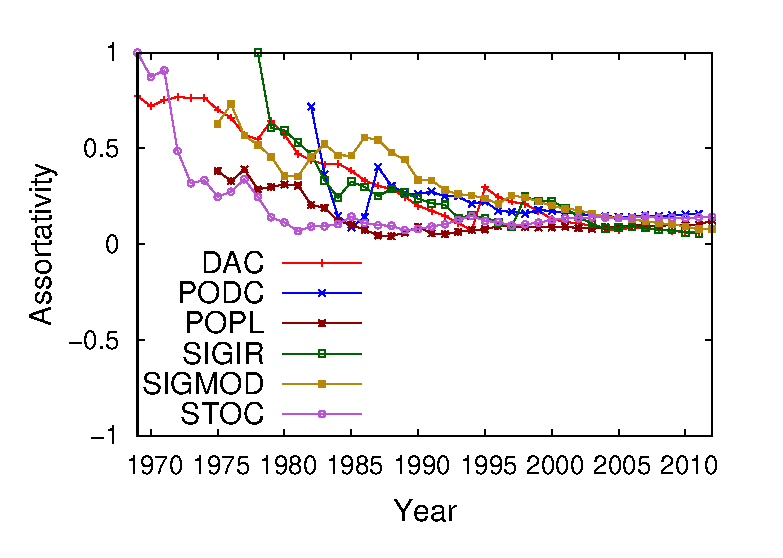
\includegraphics[scale=.33]{graficos/sigs_metricas_acumuladas_1_em_1_ano/assortatividade_grupo_temporal_web.eps}
  }%
  \subfigure[Average shortest path]{%
    \label{fig:average_shortest_path_1_in_1}
    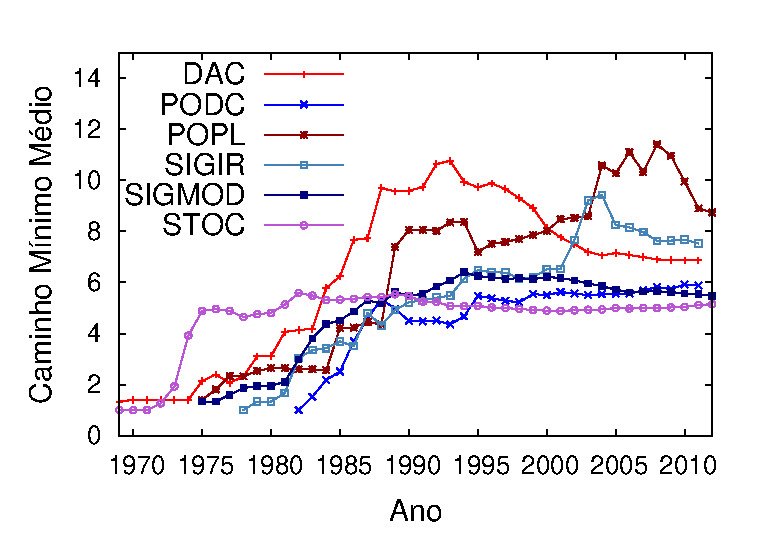
\includegraphics[scale=.33]{graficos/sigs_metricas_acumuladas_1_em_1_ano/caminho_minimo_medio_grupo_temporal_web.eps}
  }%
  \\
  \subfigure[Clustering coefficient]{%
    \label{fig:clustering_coefficient_1_in_1}
    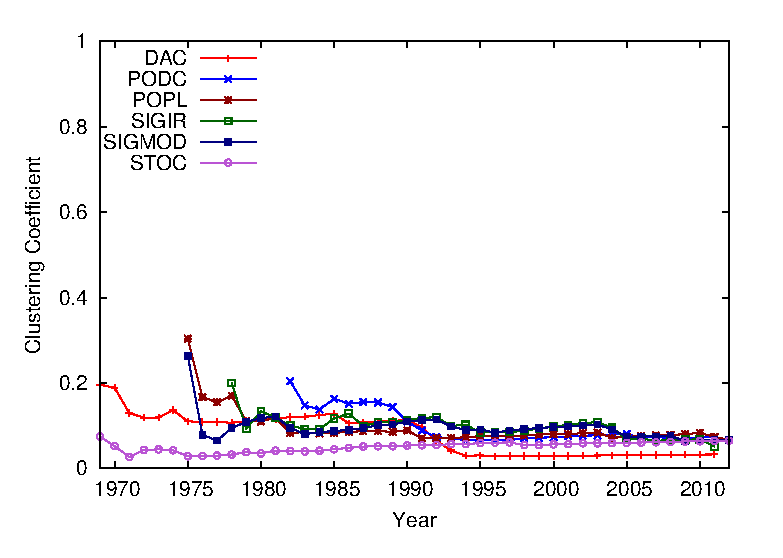
\includegraphics[scale=.33]{graficos/sigs_metricas_acumuladas_1_em_1_ano/coeficiente_agrupamento_grupo_temporal_web.eps}
  }%
  \subfigure[Largest connected component]{%
    \label{fig:largest_connected_component_1_in_1}
    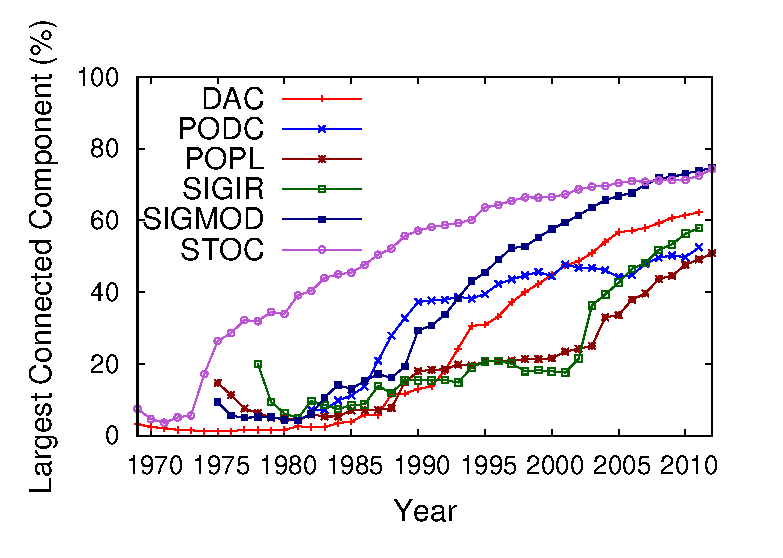
\includegraphics[scale=.33]{graficos/sigs_metricas_acumuladas_1_em_1_ano/porcentagem_maior_componente_grupo_temporal_web.eps}
  }%
  \\
  \subfigure[Average Degree - NAO CITADO NO TEXTO]{%
    \label{fig:average_degree_1_in_1}
    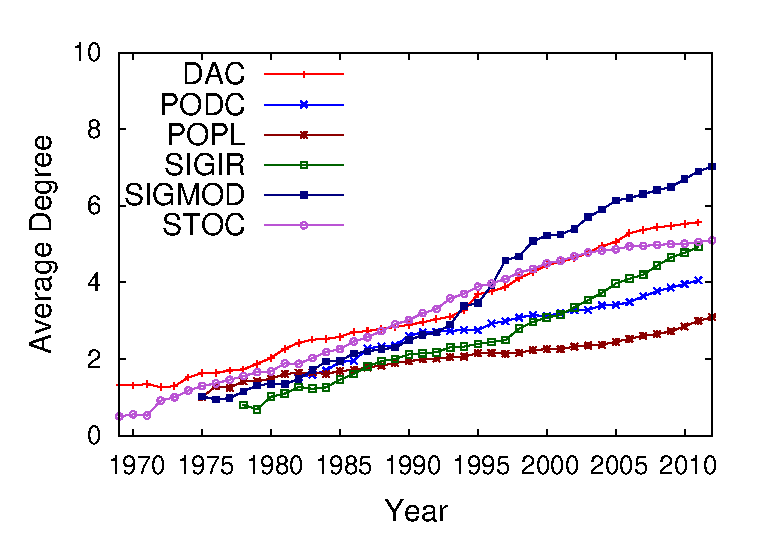
\includegraphics[scale=.33]{graficos/sigs_metricas_acumuladas_1_em_1_ano/grau_medio_nodos_grupo_temporal_web.eps}
  }%
  \end{center}
  \caption{Metrics accumulated from 1 in 1 year}
  \label{fig:metrics_accumulated_1_in_1}
\end{figure}

All in all, we can note that scientific communities have similar evolving characteristics and these properties are dynamic as they change over time.  More important, our
observations suggest that a small set authors are responsible for the social clue that create the paths among smaller and more connected research groups. Next, we seek to further
investigate this group of authors. To that end, in the next section we propose an approach to identify the author's core of scientific communities.


%\begin{figure*}
%\centering
%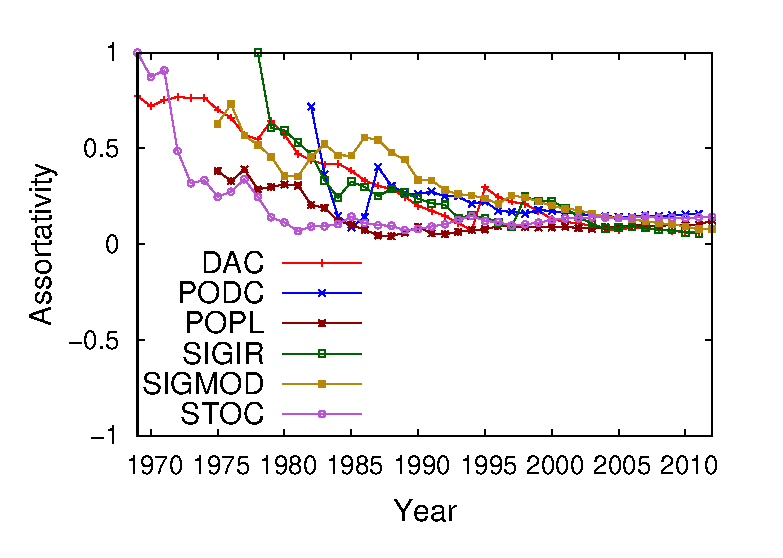
\includegraphics[scale=.4]{graficos/sigs_metricas_acumuladas_1_em_1_ano/assortatividade_grupo_temporal_web.eps}
%\caption{Assortativity accumulated from 1 in 1 year}
%\label{fig:assortativity_1_in_1}
%\end{figure*}

%\begin{figure*}
%\centering
%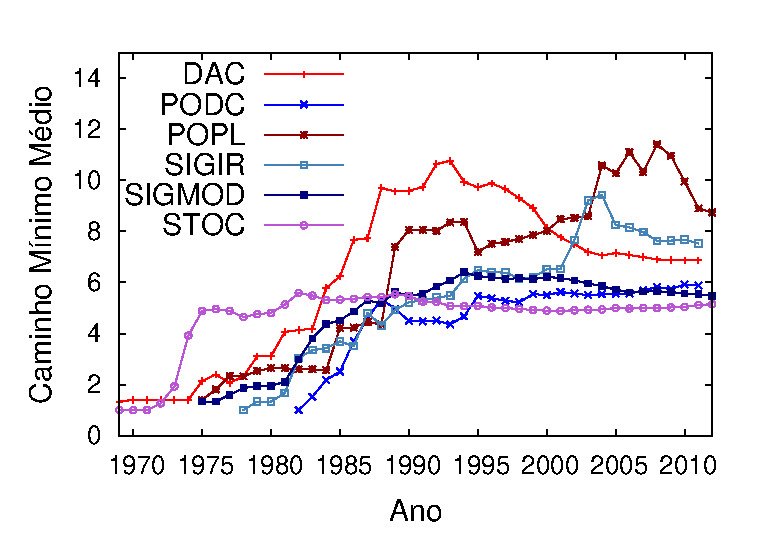
\includegraphics[scale=.4]{graficos/sigs_metricas_acumuladas_1_em_1_ano/caminho_minimo_medio_grupo_temporal_web.eps}
%\caption{Average shortest path accumulated from 1 in 1 year}
%\label{fig:average_shortest_path_1_in_1}
%\end{figure*}

%\begin{figure*}
%\centering
%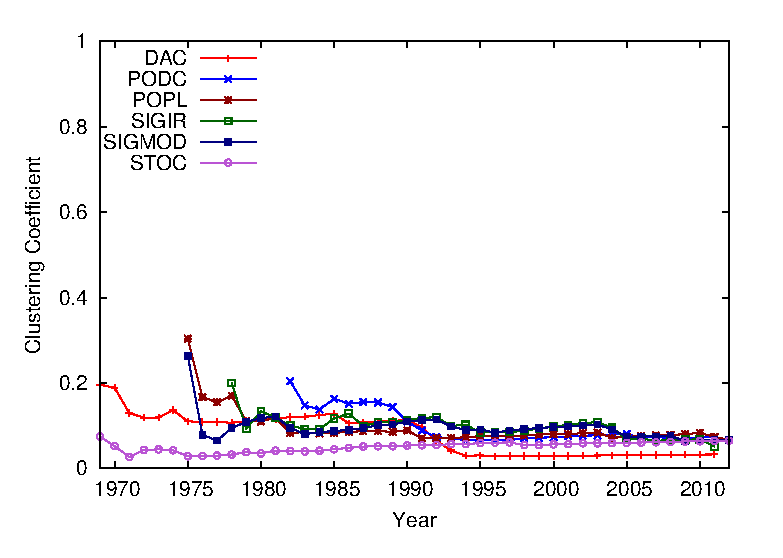
\includegraphics[scale=.4]{graficos/sigs_metricas_acumuladas_1_em_1_ano/coeficiente_agrupamento_grupo_temporal_web.eps}
%\caption{Clustering Coefficient accumulated from 1 in 1 year}
%\label{fig:clustering_coefficient_1_in_1}
%\end{figure*}

%\begin{figure*}
%\centering
%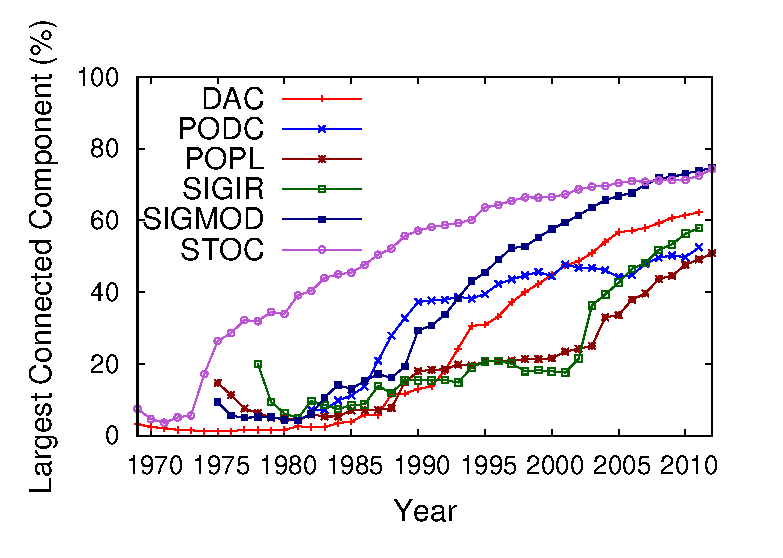
\includegraphics[scale=.4]{graficos/sigs_metricas_acumuladas_1_em_1_ano/porcentagem_maior_componente_grupo_temporal_web.eps}
%\caption{Largest connected component accumulated from 1 in 1 year}
%\label{fig:largest_connected_component_1_in_1}
%\end{figure*}




\section{Defining a Community Core}

Previous attempts for identifying the community core of a scientific community are based on algorithmic approaches that aim at identifying dense clusters of nodes in the
network~\cite{Seifi:2012:CCE:2187980.2188258}.  However, as we plan to investigate the role of a core in the network structure, any approach that makes use of the network structure
to identify such nodes could lead us to a biased set of researchers. Instead, we focus on developing a metric that quantifies the involvement of a researcher in a scientific community
during a certain period of time.  Intuitively, this metric should be able to capture (i) the prolificness of a researcher in different communities and (ii) the frequency of involvement
of that researcher with the community in a certain period of time.

First, in order to capture the prolificness of a researcher, we use the h-index~\cite{Hirsch:2005}, a metric widely adopted for this purpose. This metric consists of an index that
attempts to measure both the productivity and the impact of the published work of a researcher. It is based on the set of the researcher's most cited papers and the number of
citations that they have received.  More specifically, a researcher $a$ has an h-index $h_a$ if she has published h papers which have received at least h citations. Thus, for
example, if a researcher has 10 papers with at least 10 citations, her h-index is 10.  

Second, as an attempt to capture the importance of a researcher to a specific community in a certain period of time, we multiple her h-index by the number of publications this
researcher has in a certain community during a time window. We name this measure \textit{Core Score}. More formally, the Core Score of a researcher $r$ in a community $c$ during a period of
time $t$, $Core{ }Score_{r,c,t}$, is given by its $h\textrm{-}index_r$ multiplied by the number of publications $r$ has in $c$ during $t$ ($\textrm{\#}publications_{r,c,t}$),
as expressed by Equation~\ref{eq:core_score}. 

\begin{equation} 
  \label{eq:core_score}
  Core{ }Score_{r,c,t} = h\textrm{-}index_r \times \textrm{\#}publications_{r,c,t}
\end{equation}

%\begin{equation} 
%  \label{eq:core_score}
%  Core{ }Score_{a,c,t} = h\textrm{-}index_a \times number\textrm{ }of\textrm{ }publications_{a,c,t}
%\end{equation}

We note that the first part of the equation captures the importance of a researcher to the scientific community as a whole regardless any specific research area or period of time and the second part weights this
importance based on the activity of the researcher in a certain community and time.  By computing the core score for the members of a community, we define the community core in a
certain period of time as the top researchers of that community in terms of their core scores in the given period. Next, in Section~\ref{sub:hindex}, we detail how we inferred the
h-index of researchers. 
Then, Section~\ref{sub:thresholds} discusses how we define two important thresholds: the size of the community core and the time window used in our analyses.


\subsection{Inferring Researchers' H-index}
\label{sub:hindex}

There are multiple tools that measure the h-index of research authors, out of which Google Citations\footnote{http://scholar.google.com/citations} is the most prominent one.
However, to have a profile in this system, a researcher needs to sign up and explicitly create her research profile.  In a preliminary collection of part of the profiles of
the DBLP authors, we found that less than 30\% of these researchers had a profile at Google citations. Thus, this strategy would reduce our dataset and
potentially introduce bias when analyzing the communities.
 
To divert from this limitation, we used data from SHINE, the Simple HINdex Estimation project\footnote{http://shine.icomp.ufam.edu.br/}, to infer the researchers' h-index.
SHINE provides a website that allows users to check the h-index of almost two thousands computer science conferences. They crawled Google Scholar, searching for the title of papers
published in a number of conferences, which allowed them to effectively estimate the h-index of these target conferences based on the citations computed by Google Scholar. Although
SHINE only allows one to search for the h-index of a conference, the SHINE developers kindly allowed us to access their database to infer the h-index of researchers based on the
conferences they crawled.


\begin{figure}[!htb]
\centering
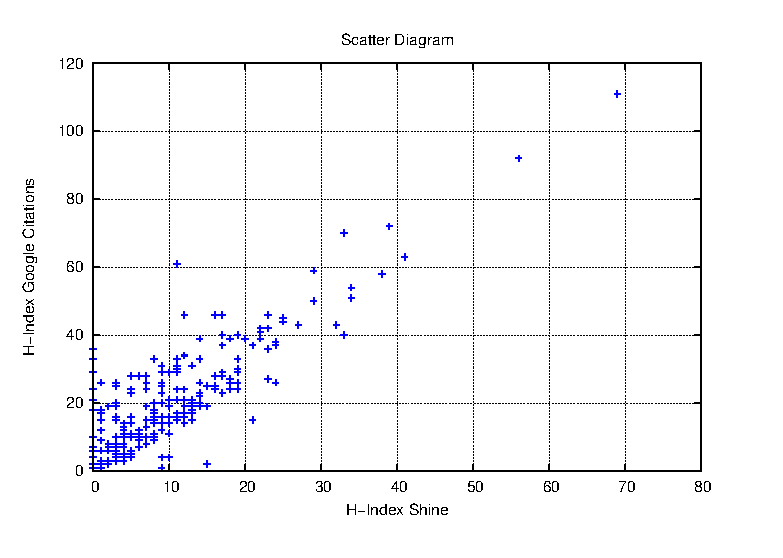
\includegraphics[scale=.5]{graficos/hindex/hindex_scatter_plot.eps}
\caption{Correlation between the inferred h-index and Google Citations one}
\label{fig:hindex_scatter_plot}
\end{figure}


However, there is one important limitation with this strategy.  As SHINE does not track all the existent computer science conferences, researchers' h-index might be underestimated when computed
with this data. To investigate this issue, we compared the h-index of a set of researchers with a profile on Google Scholar with their estimated h-index based on the SHINE data. For this, we
randomly selected 10 researchers for each conference from Table~\ref{tab:sigs_conference_period} and extracted their h-indexes from their Google Scholar profiles.  In comparison
with the h-index we estimated from SHINE, the Google scholar values are, on average, 50\% higher. Figure~\ref{fig:hindex_scatter_plot} shows the scatter plot for the two h-index
measures. We can note that although SHINE h-index is smaller, the two measures are highly correlated. The pearson correlation coefficient is 0.85, which indicates that researchers
might have proportional h-index estimations in both systems. 

\subsection{Setting the Thresholds}
\label{sub:thresholds}

Our strategy to define these two thresholds consists of varying each of them and quantifying how they impact on the changes on the members of the community core. To measure these
changes, we compute the resemblance metric, as used in~\cite{Viswanath:2009}, which measures the fraction of members in the core at time $t_0$ that remains in the core at the
time $t_1$. For each community, we varied the window size from 1 to 5 years and the size of the community core from 10\% to 60\% of the entire community.



There are two important thresholds in our approach we need to define to determine the core of a scientific community.  The first is related to the time window in which the 
community core is computed. In other words, should we compute the community core at each year, at each two years, or for a larger time window? The second threshold is related to the
size of the community core. As we define the core of a community as the top researchers in terms of their core score during a certain time window, it is important to define the
threshold for choosing the top ones.
\begin{figure}[!htb]
  \begin{center}
    \subfigure[SIGMOD]{%
      \label{fig:sigmod_slide_window_top_list}
      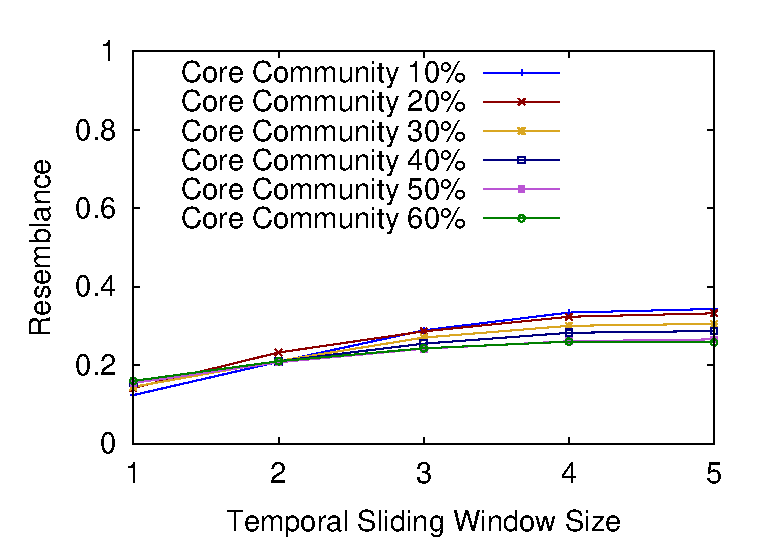
\includegraphics[scale=.33]{graficos/window_core_size/sigmod_slide_window_top_list.eps}
    }%
    \subfigure[CHI]{%
      \label{fig:chi_slide_window_top_list}
      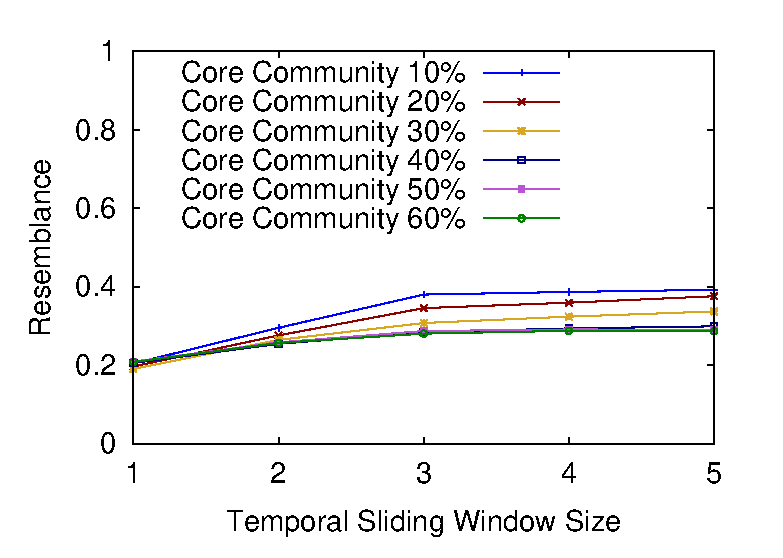
\includegraphics[scale=.33]{graficos/window_core_size/chi_slide_window_top_list.eps}
    }%
  \end{center}
\caption{Average of the values of resemblance}
 \label{fig:averange_values_resemblance}
\end{figure}


Intuitively, high resemblance variations indicate bad threshold choices and, thus, we should seek for values in which threshold changes cause slight changes on resemblance.
Figure~\ref{fig:averange_values_resemblance} shows the resemblance values as a function of the window size, providing different curves for the community core size.  We chose the
SIGMOD and CHI communities for this analysis. The rest of the communities are omitted due to lack of space, but the same observations hold for them. By visual inspection we would set the core
size as 10\% due to the proximity of the curves, and the window size as 2 or 3, as most of the communities showed a more stable resemblance after these values. To help us decide, we
computed the angular coefficient for the 10\% core size curves of each community and obtained the average angular coefficient for them.  Based on this value, we chose the window
size for our experiments as 3 years.


\subsection{Validation}

Based on the core score value, we expect that the members of the community core would be standing researchers that actively contribute with publications to a certain community.
The validation of this assumption is, by nature, subjective.  Thus, we provide next evidence that our approach correctly captures this expected characteristic.



\begin{figure}[!htb]
  \begin{center}
    \subfigure[Jon Kleinberg]{%
      \label{fig:cc_kleinberg}
      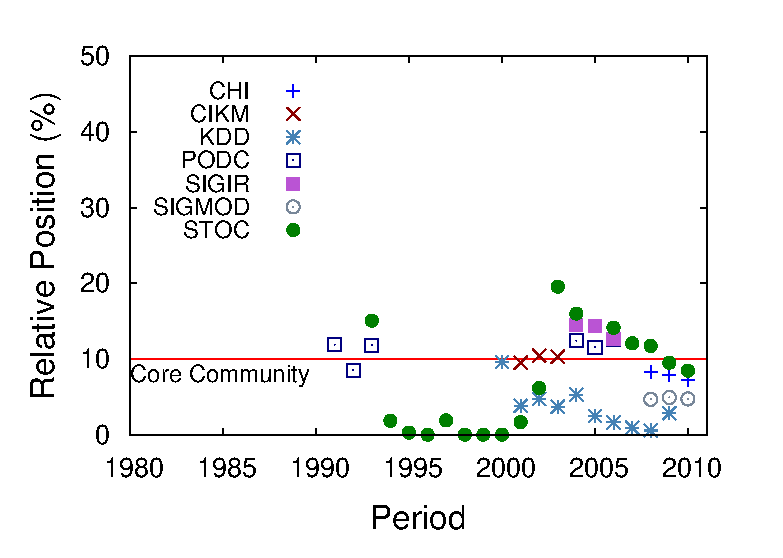
\includegraphics[scale=.33]{graficos/validacao_core_community/cc_kleinberg.eps}
    }%
    \subfigure[Luis von Ahn]{%
      \label{fig:cc_luis_von_ahn}
      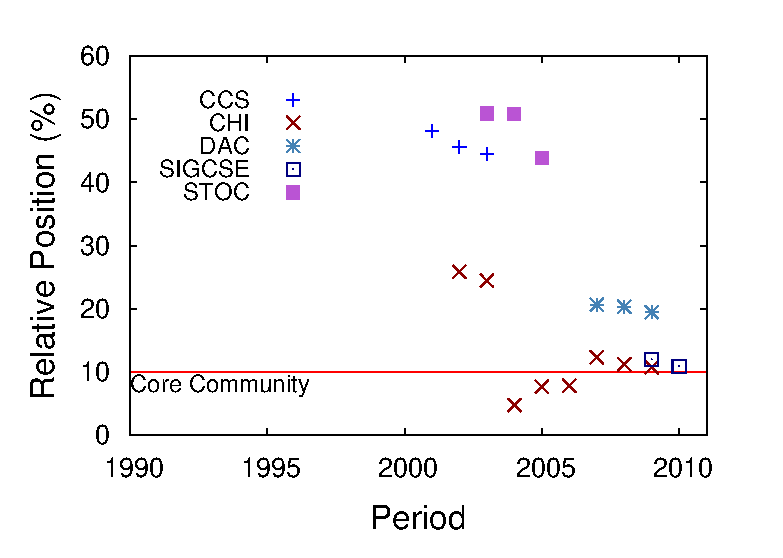
\includegraphics[scale=.33]{graficos/validacao_core_community/cc_luis_von_ahn.eps}
    }%
  \end{center}
\caption{Core score of two WWW 2013 keynote speakers}
 \label{fig:rank_core_score_authors}
\end{figure}


First, we analyzed the core score of two WWW 2013 keynote speakers: Jon Kleinberg and Luis von Ahn.  Figure~\ref{fig:rank_core_score_authors} shows the ranking position in terms of
percentage (e.g., position 5\% of that community) of these two researchers in the communities they have published. The botton line divides the members of the community core from the others.
We can note that Jon Kleinberg was a member of the community core of STOC, a theoretical conference, for years. More precisely, he was part of the STOC core for twelve years,
publishing seven STOC papers in a single period of three years. With Kleinberg's involvement on KDD, he became less active in STOC and left the core of that community for some time.
During this period, he published several KDD papers, while his STOC publications were drastically reduced.  When it comes to Luis von Ahn, we can note that he is more active in
the CHI community, a community in which he published six papers along his academic life. He reached the core of the CHI community along three consecutive time windows,
publishing four CHI papers in a single period.




\begin{table*}[!hptb]
\centering
\caption{Researchers who appear most often in the community core over the years}
\label{tab:authors_frequency_core_community}
{\small
\begin{tabular}{|c|c|c|c|} \hline
\bf{KDD} & \bf{SIGCOMM} & \bf{SIGIR} & \bf{SIGMOD}\\ \hline
Heikki Mannila$^\star$ & Scott Shenker$^\star$ & W. Bruce Croft$^\star$ & David J. DeWitt$^\star$\\ \hline
Jiawei Han$^\star$ & George Varghese & Clement T. Yu & Michael Stonebraker$^\star$\\ \hline
Eamonn J. Keogh & Hui Zhang & Susan T. Dumais$^\star$ & H. V. Jagadish\\ \hline
Martin Ester & Donald F. Towsley$^\star$ & James Allan & Rakesh Agrawal$^\star$\\ \hline
Bing Liu & Hari Balakrishnan & Justin Zobel & Christos Faloutsos\\ \hline
Padhraic Smyth$^\star$ & Ion Stoica & Alistair Moffat & Raghu Ramakrishnan\\ \hline
Charu C. Aggarwal & Srinivasan Seshan & Norbert Fuhr$^\star$ & Jiawei Han\\ \hline
Philip S. Yu & Deborah Estrin & James P. Callan & Gerhard Weikum\\ \hline
Ke Wang & David Wetherall & Yiming Yang & Philip A. Bernstein$^\star$\\ \hline
Hans-Peter Kriegel & Thomas E. Anderson & Edward A. Fox & Jeffrey F. Naughton\\ \hline
Rakesh Agrawal$^\star$ & Jennifer Rexford & Gerard Salton$^\star$ & Hector Garcia-Molina$^\star$\\ \hline
Jian Pei & Jia Wang & Ricardo A. Baeza-Yates & Michael J. Carey$^\star$\\ \hline
Wynne Hsu & Ratul Mahajan & Jian-Yun Nie & Joseph M. Hellerstein\\ \hline
Qiang Yang & Vern Paxson$^\star$ & Mark Sanderson & Philip S. Yu\\ \hline
Christos Faloutsos$^\star$ & Mark Handley & Charles L. A. Clarke & Divesh Srivastava\\ \hline
Huan Liu & Yin Zhang & Chris Buckley & Michael J. Franklin\\ \hline
Mohammed Javeed Zaki & Peter Steenkiste & Chengxiang Zhai & Jennifer Widom$^\star$\\ \hline
Pedro Domingos & Walter Willinger & Alan F. Smeaton & Hans-Peter Kriegel\\ \hline
Jon M. Kleinberg & Ramesh Govindan & Zheng Chen & Hamid Pirahesh\\ \hline
Vipin Kumar$^\star$ & Jon Crowcroft$^\star$ & Ophir Frieder & Surajit Chaudhuri$^\star$\\ \hline
\end{tabular}
\par\medskip\footnotesize{$^\star$ Researchers awarded by a lifetime of innovation and leadership inside that community.}
}
\end{table*}




Next, we computed a ranking of researchers that appear most often in the community core of each scientific community. We chose the KDD, SIGCOMM, SIGIR, and SIGMOD communities to
show their top 20 researchers in Table~\ref{tab:authors_frequency_core_community}.  As we can note, several big names appear in this top list, including past keynote speakers of
these conferences as well as awarded researchers by their life time contributions in that community. Indeed, by analyzing the awarded researchers from each community we found that
a large fraction of them appeared in the community core at least one time in the conference history. More specifically, these fractions are 75\% of the awarded
KDD\footnote{http://www.sigkdd.org/awards\_innovation.php} members, 35\% for SIGCOMM\footnote{http://www.sigcomm.org/awards/sigcomm-awards}, 60\% for
SIGIR\footnote{http://www.sigir.org/awards/awards.html}, and 80\% for SIGMOD\footnote{http://www.sigmod.org/sigmod-awards}.  Except for SIGCOMM, a community with many sponsored
event that were not considered in our datasets, the other three communities presented very high numbers of awarded members that appear at least one time a community core. These
observations provide evidence that our approach correctly captures the notion of a scientific community core.








%\begin{tabular}{|c|l|l|l|l|} \hline
% & \bf{KDD} & \bf{SIGCOMM} & \bf{SIGIR} & \bf{SIGMOD}\\ \hline
%1\textsuperscript{st} & Heikki Mannila$^\star$ & Scott Shenker$^\star$ & W. Bruce Croft$^\star$ & David J. DeWitt$^\star$\\ \hline
%2\textsuperscript{nd} & Jiawei Han$^\star$ & George Varghese & Clement T. Yu & Michael Stonebraker$^\star$\\ \hline
%3\textsuperscript{rd} & Eamonn J. Keogh & Hui Zhang & Susan T. Dumais$^\star$ & H. V. Jagadish\\ \hline
%4\textsuperscript{th} & Martin Ester & Donald F. Towsley$^\star$ & James Allan & Rakesh Agrawal$^\star$\\ \hline
%5\textsuperscript{th} & Bing Liu & Hari Balakrishnan & Justin Zobel & Christos Faloutsos\\ \hline
%6\textsuperscript{th} & Padhraic Smyth$^\star$ & Ion Stoica & Alistair Moffat & Raghu Ramakrishnan\\ \hline
%7\textsuperscript{th} & Charu C. Aggarwal & Srinivasan Seshan & Norbert Fuhr$^\star$ & Jiawei Han\\ \hline
%8\textsuperscript{th} & Philip S. Yu & Deborah Estrin & James P. Callan & Gerhard Weikum\\ \hline
%9\textsuperscript{th} & Ke Wang & David Wetherall & Yiming Yang & Philip A. Bernstein$^\star$\\ \hline
%10\textsuperscript{th} & Hans-Peter Kriegel & Thomas E. Anderson & Edward A. Fox & Jeffrey F. Naughton\\ \hline
%11\textsuperscript{th} & Rakesh Agrawal$^\star$ & Jennifer Rexford & Gerard Salton$^\star$ & Hector Garcia-Molina$^\star$\\ \hline
%12\textsuperscript{th} & Jian Pei & Jia Wang & Ricardo A. Baeza-Yates & Michael J. Carey$^\star$\\ \hline
%13\textsuperscript{th} & Wynne Hsu & Ratul Mahajan & Jian-Yun Nie & Joseph M. Hellerstein\\ \hline
%14\textsuperscript{th} & Qiang Yang & Vern Paxson$^\star$ & Mark Sanderson & Philip S. Yu\\ \hline
%15\textsuperscript{th} & Christos Faloutsos$^\star$ & Mark Handley & Charles L. A. Clarke & Divesh Srivastava\\ \hline
%16\textsuperscript{th} & Huan Liu & Yin Zhang & Chris Buckley & Michael J. Franklin\\ \hline
%17\textsuperscript{th} & Mohammed Javeed Zaki & Peter Steenkiste & Chengxiang Zhai & Jennifer Widom$^\star$\\ \hline
%18\textsuperscript{th} & Pedro Domingos & Walter Willinger & Alan F. Smeaton & Hans-Peter Kriegel\\ \hline
%19\textsuperscript{th} & Jon M. Kleinberg & Ramesh Govindan & Zheng Chen & Hamid Pirahesh\\ \hline
%20\textsuperscript{th} & Vipin Kumar$^\star$ & Jon Crowcroft$^\star$ & Ophir Frieder & Surajit Chaudhuri$^\star$\\ \hline
%\end{tabular}
%}
% \par\medskip\footnotesize{$^\star$ Researchers awarded by a lifetime of innovation and leadership inside that community.}
%\end{table*}
% \let\thefootnote\relax\footnote{$^\star$ Researchers awarded by a lifetime of innovation and leadership inside that community.}
%  & \bf CIKM & \bf KDD &\bf  SIGIR & \bf SIGMOD\\ \hline
% 1\textsuperscript{st} & Philip S. Yu & Heikki Mannila & W. Bruce Croft* & David J. DeWitt*\\ \hline
% 2\textsuperscript{nd} & Jiawei Han & Jiawei Han & Clement T. Yu & Michael Stonebraker*\\ \hline
% 3\textsuperscript{rd} & Ling Liu & Eamonn J. Keogh & Susan T. Dumais* & H. V. Jagadish\\ \hline
% 4\textsuperscript{th} & Clement T. Yu & Martin Ester & James Allan & Rakesh Agrawal*\\ \hline
% 5\textsuperscript{th} & Christos Faloutsos & Bing Liu & Justin Zobel & Christos Faloutsos\\ \hline
% 6\textsuperscript{th} & James Allan & Padhraic Smyth & Alistair Moffat & Raghu Ramakrishnan\\ \hline
% 7\textsuperscript{th} & Elke A. Rundensteiner & Charu C. Aggarwal & Norbert Fuhr* & Jiawei Han\\ \hline
% 8\textsuperscript{th} & Ke Wang & Philip S. Yu & James P. Callan & Gerhard Weikum\\ \hline
% 9\textsuperscript{th} & Amr El Abbadi & Ke Wang & Yiming Yang & Philip A. Bernstein*\\ \hline
% 10\textsuperscript{th} & W. Bruce Croft & Hans-Peter Kriegel & Edward A. Fox & Jeffrey F. Naughton\\ \hline
% 11\textsuperscript{th} & Ming-Syan Chen & Rakesh Agrawal & Gerard Salton* & Hector Garcia-Molina*\\ \hline
% 12\textsuperscript{th} & Divyakant Agrawal & Jian Pei & Ricardo A. Baeza-Yates & Michael J. Carey*\\ \hline
% 13\textsuperscript{th} & C. Lee Giles & Wynne Hsu & Jian-Yun Nie & Joseph M. Hellerstein\\ \hline
% 14\textsuperscript{th} & Weiyi Meng & Qiang Yang & Mark Sanderson & Philip S. Yu\\ \hline
% 15\textsuperscript{th} & Berthier A. Ribeiro-Neto & Christos Faloutsos & Charles L. A. Clarke & Divesh Srivastava\\ \hline
% 16\textsuperscript{th} & M. Tamer \"Ozsu & Huan Liu & Chris Buckley & Michael J. Franklin\\ \hline
% 17\textsuperscript{th} & ChengXiang Zhai & Mohammed Javeed Zaki & ChengXiang Zhai & Jennifer Widom*\\ \hline
% 18\textsuperscript{th} & Javed A. Aslam & Pedro Domingos & Alan F. Smeaton & Hans-Peter Kriegel\\ \hline
% 19\textsuperscript{th} & Hans-Peter Kriegel & Jon M. Kleinberg & Zheng Chen & Hamid Pirahesh\\ \hline
% 20\textsuperscript{th} & Bing Liu & Vipin Kumar & Ophir Frieder & Surajit Chaudhuri*\\ \hline

\section{Properties of Community Cores}

In this section, we present a series of analyses about the scientific community cores. First, we analyze how the network properties of the scientific communities have evolved. 
Then, we contrast the properties of the community cores over time against the properties of the remaining members of the respective communities. 
Finally, we compute the average core score of a community to investigate fluctuations in the properties of the members of the community cores and 
correlate these fluctuations with the network properties of the communities.


\subsection{Evolution of the Scientific Communities}
\label{sub:time}

In order to study the evolution of the main structural properties of the scientific communities, we examine 
various network metrics for each of the scientific communities. We present four popular metrics here: assortativity, clustering coefficient (CC), average shortest path (ASP), 
and the size of the largest weakly connected component (WCC). Figure~\ref{fig:metrics} shows how each of these four metrics vary over time
for a set of six scientific communities selected among those that span over the longest period in our dataset.  Our analyses are performed under two perspectives. The first
consists on analyzing the network evolution year by year by accumulating nodes and edges to a single final snapshot of the graph. This perspective allows us to observe the final
network structure of a community as a function of time. The second perspective consists of analyzing snapshots constructed based on nodes and edges created on a predefined time
window (three years, as discussed in Subsection~\ref{sub:thresholds}). This analysis allows us to investigate network variations with potential to impact the final network structure.
Our analysis results are similar for the other communities, but we omit them due to lack of space.



\begin{figure}[!htb]
  \vspace{-0.2cm}
  \begin{center}
  \subfigure[Final Assortativity]{%
    \label{fig:assortativity_1_in_1}
    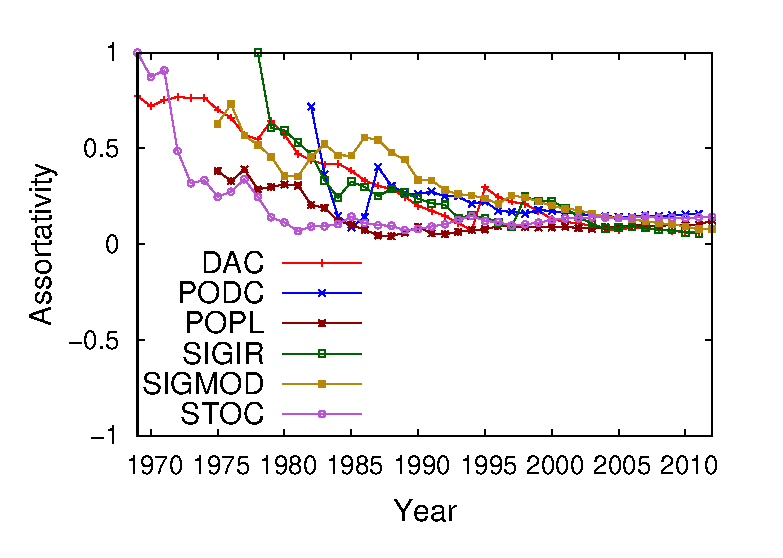
\includegraphics[scale=.33]{graficos/sigs_metricas_acumuladas_1_em_1_ano/assortatividade_grupo_temporal_web.eps}
  }%
  \subfigure[Assortativity per Window]{%
    \label{fig:assortativity_slide_window}
    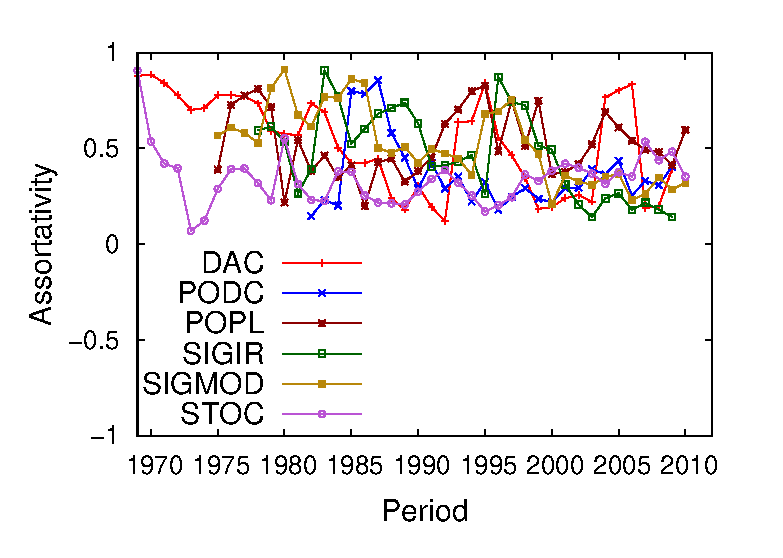
\includegraphics[scale=.33]{graficos/core_over_time/metricas_tradicionais/assortatividade_slide_window_grupo_temporal_web.eps}
  }%
  \\
  \subfigure[Final ASP]{%
    \label{fig:average_shortest_path_1_in_1}
    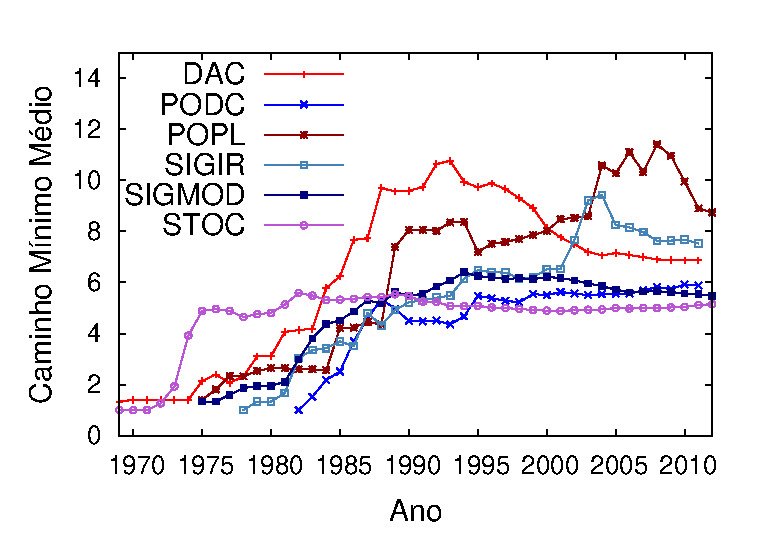
\includegraphics[scale=.33]{graficos/sigs_metricas_acumuladas_1_em_1_ano/caminho_minimo_medio_grupo_temporal_web.eps}
  }%
  \subfigure[ASP per Window]{%
    \label{fig:average_shortest_path_slide_window}
    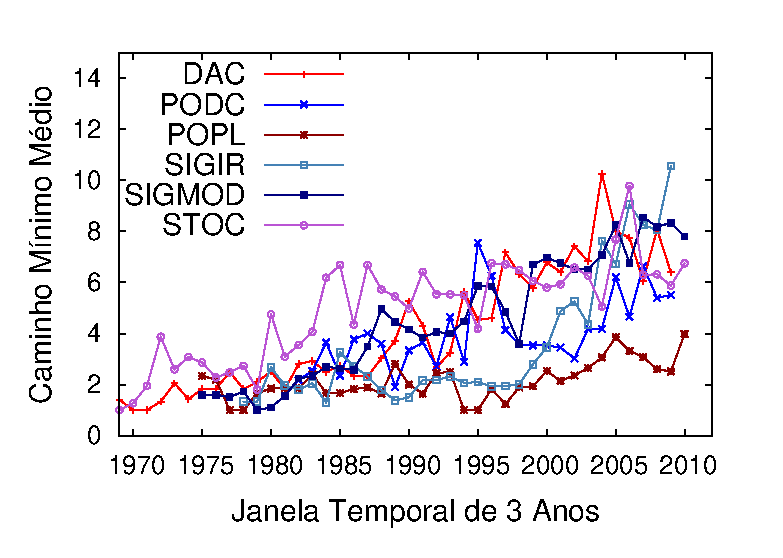
\includegraphics[scale=.33]{graficos/core_over_time/metricas_tradicionais/caminho_minimo_medio_slide_window_grupo_temporal_web.eps}
  }%
  \\
  \subfigure[Final CC]{%
    \label{fig:clustering_coefficient_1_in_1}
    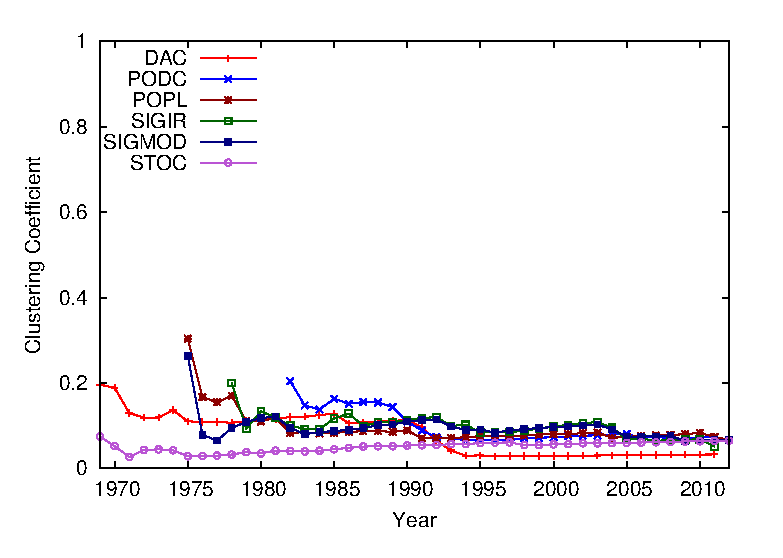
\includegraphics[scale=.33]{graficos/sigs_metricas_acumuladas_1_em_1_ano/coeficiente_agrupamento_grupo_temporal_web.eps}
  }%
  \subfigure[CC per Window]{%
    \label{fig:clustering_coefficient_slide_window}
    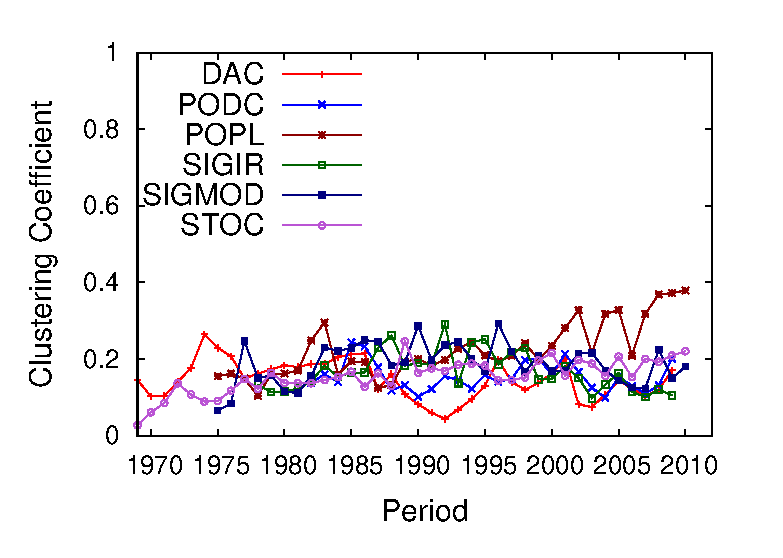
\includegraphics[scale=.33]{graficos/core_over_time/metricas_tradicionais/coeficiente_agrupamento_slide_window_grupo_temporal_web.eps}
  }%
  \\
  \subfigure[Final Largest WCC]{%
    \label{fig:largest_connected_component_1_in_1}
    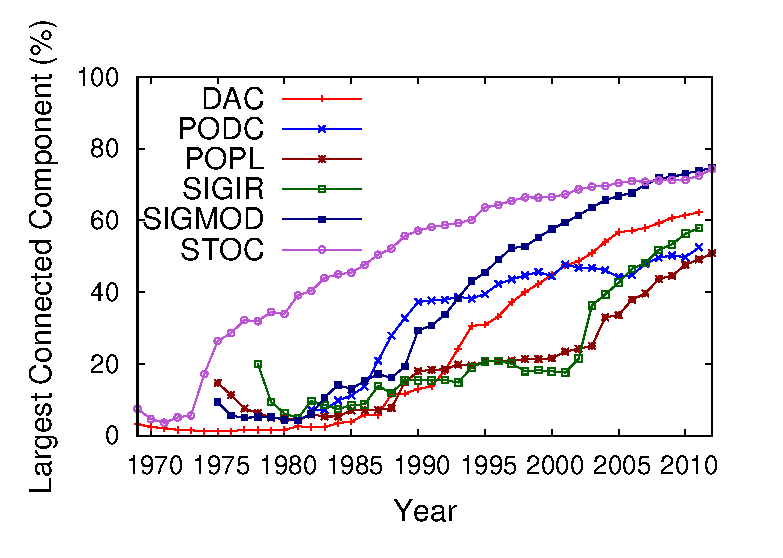
\includegraphics[scale=.33]{graficos/sigs_metricas_acumuladas_1_em_1_ano/porcentagem_maior_componente_grupo_temporal_web.eps}
  }%
  \subfigure[Largest WCC per Window]{%
    \label{fig:largest_connected_component_slide_window}
    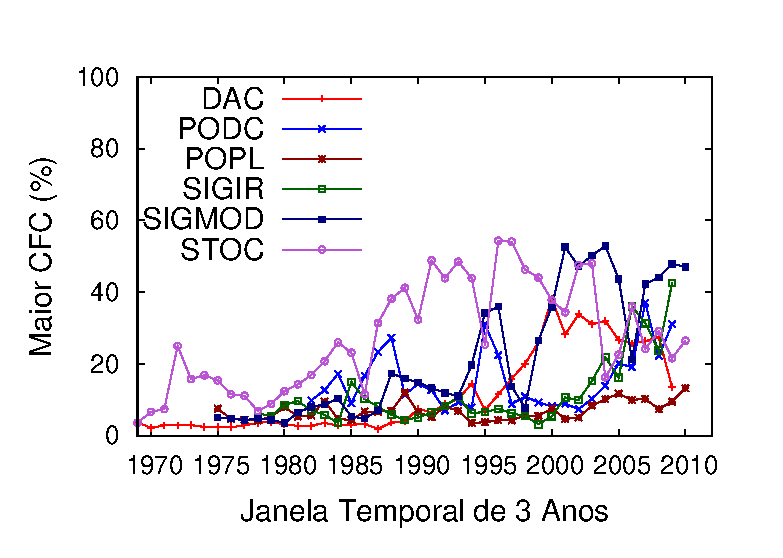
\includegraphics[scale=.33]{graficos/core_over_time/metricas_tradicionais/porcentagem_maior_componente_slide_window_grupo_temporal_web.eps}
  }%
  \\
  \subfigure[Final Average Degree]{%
    \label{fig:average_degree_1_in_1}
    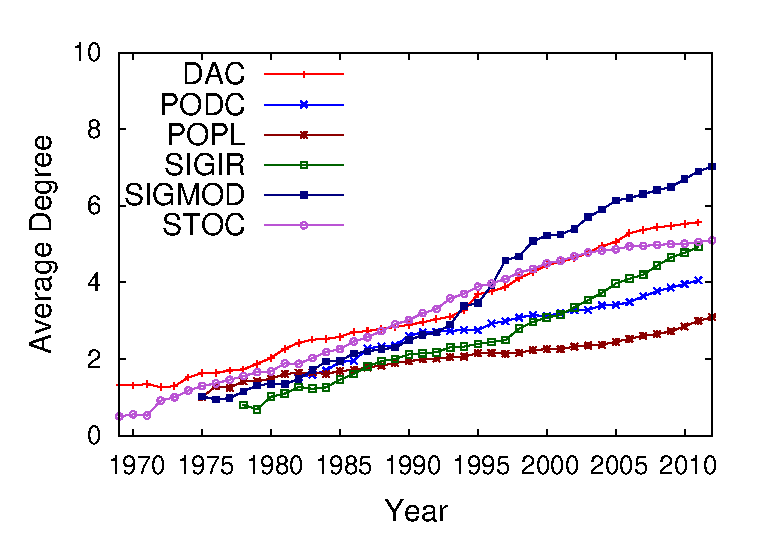
\includegraphics[scale=.33]{graficos/sigs_metricas_acumuladas_1_em_1_ano/grau_medio_nodos_grupo_temporal_web.eps}
  }%
  \subfigure[Avg. Degree per Window]{%
    \label{fig:average_degree_slide_window}
    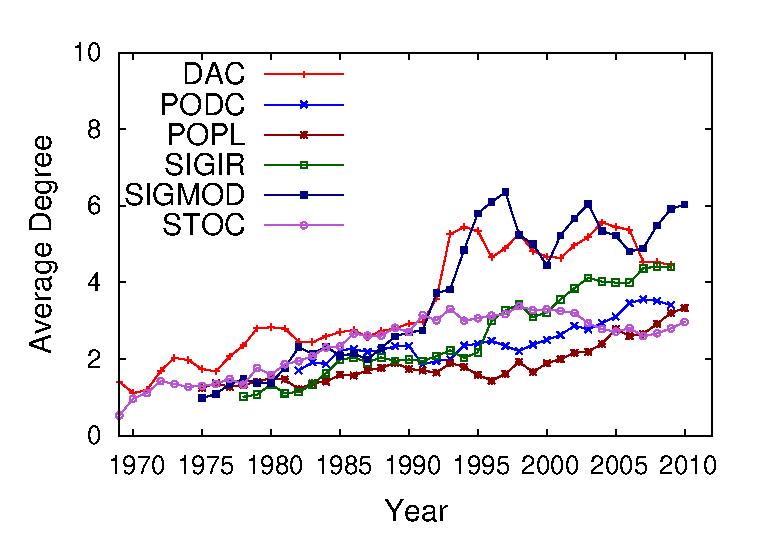
\includegraphics[scale=.33]{graficos/core_over_time/metricas_tradicionais/grau_medio_nodos_slide_window_grupo_temporal_web.eps}
  }%
  \end{center}
  \vspace{-0.5cm}
  \caption{Network evolution metrics for scientific communities}
  \vspace{-0.5cm}
  \label{fig:metrics}
\end{figure}


We note from Figure~\ref{fig:metrics} that the largest WCC tend to largely increase as a function of time. This suggests that at early
stages, scientific communities are formed by several small and segregated research groups. With time, some researchers (e.g., students) leave their institutions and begin collaborations
with other research groups. Additionally, as the community evolves, heads of  research groups tend to collaborate with other peers of the same community. Thus, with time, researchers
from different groups tend to collaborate and increase the size of the largest WCC. As a consequence, the average shortest path, computed only on the largest
WCC, tends to increase, becoming stable around typical small-world values (i.e., from 4 to 10 hops)~\cite{mislove-2007-socialnetworks,fourdegrees_facebook}.  We can
also note that the average clustering coefficient tends to values between 0.1 and 0.2, thus suggesting that the coauthors of a researcher have 10\% to 20\% of chance to be connected
among themselves. These values tend to slightly diminish over time, as small components tend to connect to form larger components reducing the average clustering coefficient
value.  When it comes to assortativity, we see that this measure tends to 0, but it is still positive. This means that there is a slight tendency in these communities of nodes to
connect with others with similar degree.  A positive value for assortativity is a typical characteristic of sociological networks~\cite{Newman2003}.

In general, we can note that scientific communities have similar evolving characteristics and these properties are dynamic as they change over time.  More important, our
observations suggest that a small set of core researchers are responsible for the social clue that creates the paths among smaller and more connected research groups. In order to 
further investigate these core researchers in the next subsection we contrast members and non-members of the community core. 







\subsection{Core Members vs. Non-Members}
\label{sub:vs}

\textit{To what extend the properties of the community core differ from the rest of the community?}  To answer this question, we compute node network properties for members and non-members of the community
core. We consider the time window analysis to understand the variations that these two classes might have in the global measure.
Figure~\ref{fig:metrics_comparing_core_community} shows the average degree and the average clustering coefficient computed by the members and non-members of the SIGMOD 
community core. Additionally, we also measure the fraction of community core members as well as non-members that are in the largest WCC and compute the average betweenness of
each of these group of members. 

We can make key observations
from theses analysis. First, we can note that the average degree of the members of the community core is considerably higher in comparison with non-members, as they tend to establish more and
more connections as a function of time. However, the clustering coefficient of the members of the community core tend to be slightly smaller in comparison with non-members meaning that they
might act like hubs, by connecting different groups with small intersection. By analyzing the fraction of members of the community core that are part of the largest
WCC, we can note that it is much larger than the fraction of non-members, suggesting that they might be connecting smaller components. 
We confirm these observations by analyzing the betweenness centrality of these groups of researchers. We can note that the average betweenness of the community core is much higher,
meaning that a higher number of shortest paths include these nodes. 

Next, we investigate how aspects of the members of a community core can impact on the overall structure of the community.


\begin{figure}[!htpb]
  \begin{center}
  \subfigure[Clustering Coefficient]{%
    \label{fig:core_com_sigmod_clustering_coefficient}
    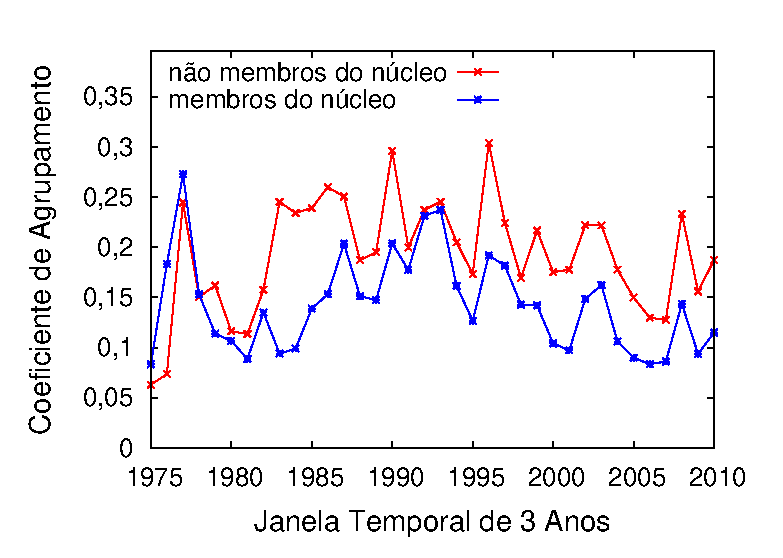
\includegraphics[scale=.31]{graficos/core_over_time/core_community/sigmod_janela_3_core_coeficiente_agrupamento.eps}
  }
  \subfigure[Avg. Degree]{%
    \label{fig:core_com_sigmod_average_degree}
    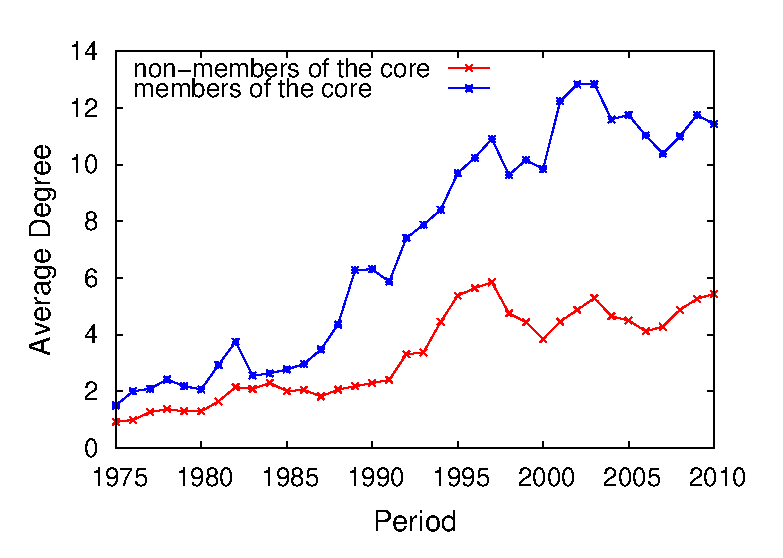
\includegraphics[scale=.31]{graficos/core_over_time/core_community/sigmod_janela_3_core_grau_medio_nodos.eps}
  }
  \\
  \subfigure[Largest WCC]{%
    \label{fig:core_com_sigmod_largest_connected_component}
    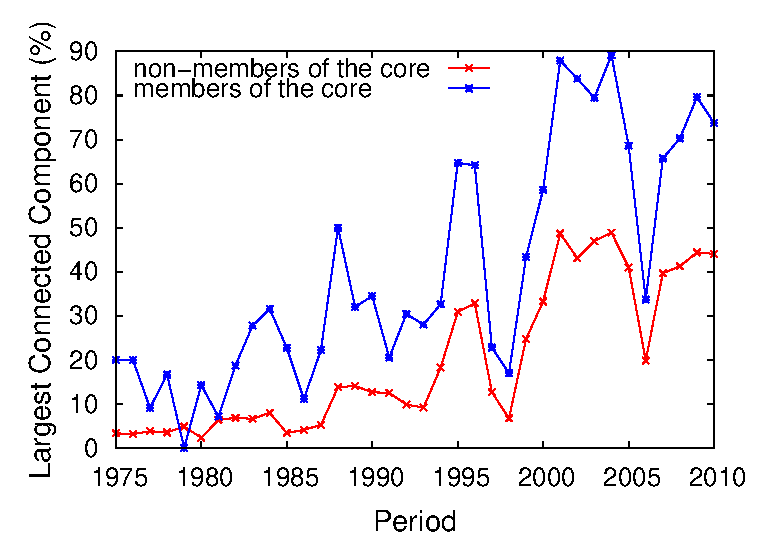
\includegraphics[scale=.31]{graficos/core_over_time/core_community/sigmod_janela_3_core_maior_componente_conectado.eps}
  }
  \subfigure[Avg. Betweenness]{%
    \label{fig:core_com_sigmod_betweenness}
    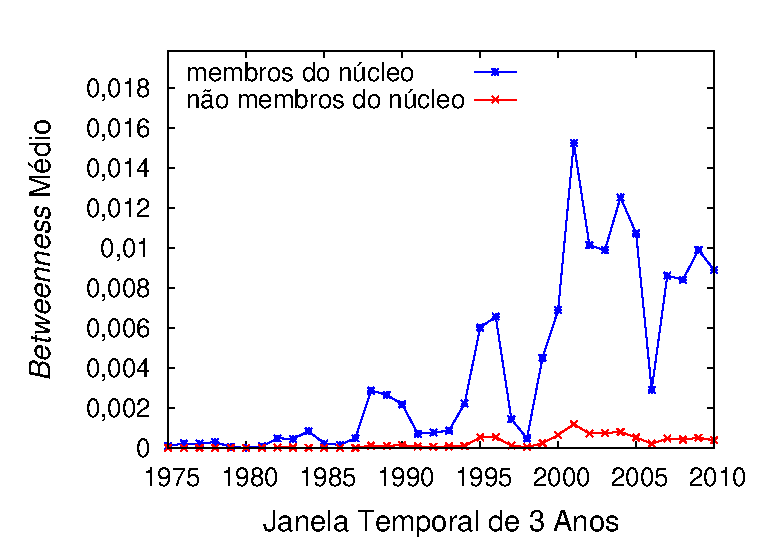
\includegraphics[scale=.31]{graficos/core_over_time/core_community/sigmod_janela_3_core_betweenness.eps}
  }
  \end{center}
  \vspace{-0.5cm}
  \caption{SIGMOD network properties for members and non-members of the core}
  \label{fig:metrics_comparing_core_community}
\end{figure}



\subsection{Community Core vs. Network Structure}
\label{sub:corr}

\begin{table*}[!htbp]
\centering
\caption{Correlation between the average core score of the community cores and the network metrics}
\label{tab:correlation_metrics}
{\small
\begin{tabular}{|l|c|c|c|c|c|c|} \hline
\bf Community & \bf Diameter & \bf Avg. Short P. & \bf Clus. Coef. & \bf Assort. & \bf Larg. WCC & \bf Avg. Deg. \\ \hline
CCS & 0.34 & 0.2 & 0.23 & -0.2 & 0.45 & 0.14 \\ \hline
CHI & 0.75 & 0.79 & -0.62 & -0.74 & 0.76 & 0.77 \\ \hline
CIKM & 0.56 & 0.56 & -0.52 & -0.67 & 0.39 & 0.87 \\ \hline
DAC & 0.8 & 0.85 & -0.49 & -0.63 & 0.76 & 0.92 \\ \hline
HSCC & 0.17 & 0.45 & -0.62 & -0.71 & 0.87 & 0.55 \\ \hline
ICSE & 0.81 & 0.83 & -0.52 & -0.84 & 0.68 & 0.8 \\ \hline
ISCA & 0.63 & 0.55 & 0.54 & -0.32 & 0.63 & 0.81  \\ \hline
ISSAC & 0.05 & 0.01 & -0.25 & -0.43 & -0.07 & 0.21 \\ \hline
KDD & 0.1 & 0.17 & -0.33 & -0.67 & 0.2 & 0.14\\ \hline
MICRO & 0.35 & 0.35 & 0.28 & -0.36 & 0.52 & 0.51 \\ \hline
MOBICOM & -0.04 & 0.11 & 0.13 & -0.65 & 0.23 & -0.09 \\ \hline
MM & 0.67 & 0.68 & -0.91 & -0.95 & 0.67 & 0.69 \\ \hline
PODC & 0.4 & 0.42 & -0.23 & -0.2 & 0.13 & 0.68 \\ \hline
POPL & 0.21 & 0.2 & 0.23 & -0.43 & 0.25 & 0.19 \\ \hline
SAC & 0.48 & 0.59 & 0.16 & -0.39 & -0.55 & 0.16 \\ \hline
SIGCOMM & 0.18 & 0.19 & 0.05 & -0.81 & 0.49 & 0.41\\ \hline
SIGCSE & 0.88 & 0.84 & -0.22 & -0.5 & 0.93 & 0.87 \\ \hline
SIGDOC & 0.73 & 0.78 & -0.36 & -0.89 & 0.66 & 0.76 \\ \hline
SIGGRAPH & 0.79 & 0.85 & -0.45 & -0.75 & 0.94 & 0.88 \\ \hline
SIGIR & 0.83 & 0.85 & -0.42 & -0.77 & 0.7 & 0.89 \\ \hline
SIGMETRICS & 0.31 & 0.24 & 0.3 & -0.44 & 0.37 & 0.64 \\ \hline
SIGMOD & 0.78 & 0.81 & 0.27 & -0.61 & 0.77 & 0.87 \\ \hline
SIGUCCS & 0.38 & -0.22 & 0.53 & -0.13 & 0.51 & 0.7 \\ \hline
STOC & 0.61 & 0.63 & 0.54 & -0.37 & 0.82 & 0.88\\ \hline \hline
{\bf Average} & {\bf 0.49} & {\bf 0.49} & {\bf -0.11} & {\bf -0.56} & {\bf 0.5} & {\bf 0.59} \\ \hline
\end{tabular}
}
\end{table*}


We now examine to what extent the community core fluctuations affect the network structure.  To that end, we compute the average core score of the members of each community over
time. Intuitively, this measure captures the overall prolificness and involvement of the core members of a scientific community. Figure~\ref{fig:average_core_score} shows this value
for a set of communities as a function of time. We plot it in two separate figures to facilitate visualization. We can note that all communities experimented rises and falls along
its life time, indicating strong variations in the core score values of the core members. We can speculate innumerous factors that are able to explain such variations,
including expansion or reduction in the number of published papers, raise and fall of hot topics with ability to attract or loose important core members, members involved in the
conference organization, etc. However, disregarding what caused these variations, we want to investigate if such variations can directly impact the network structure.


\begin{figure}[!htb]
  \begin{center}
    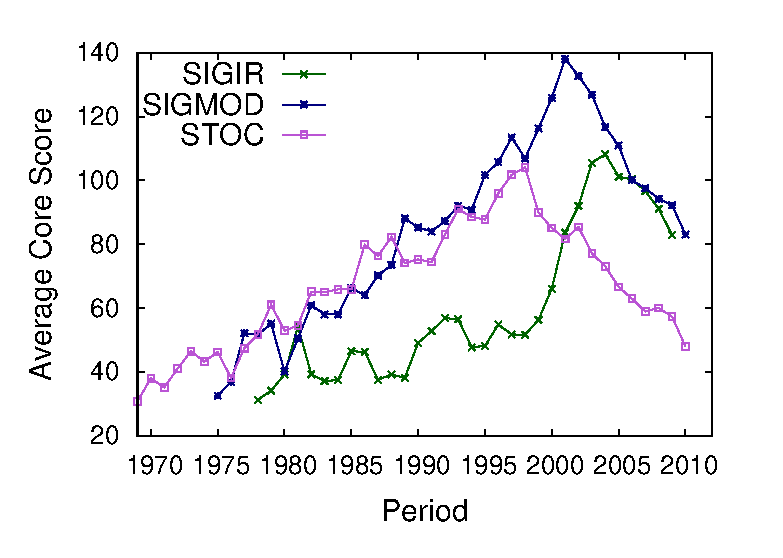
\includegraphics[scale=.325]{graficos/average_core_score/average_core_score_slide_window_grupo_1_temporal_web.eps}
    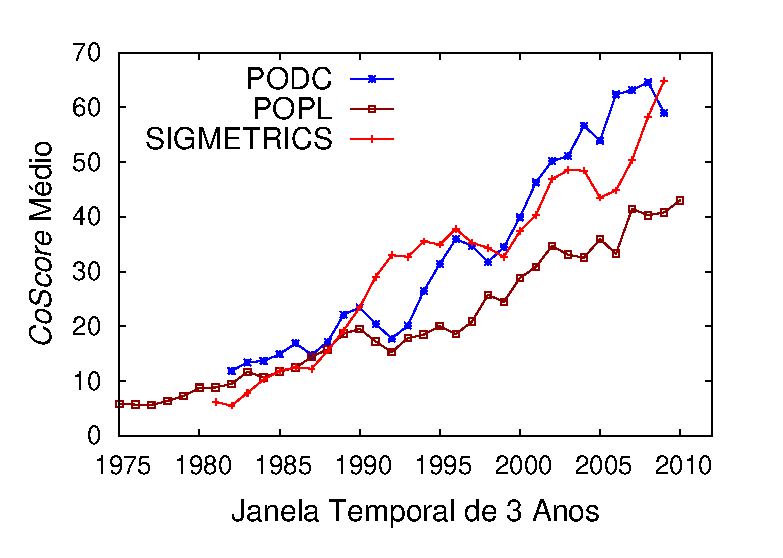
\includegraphics[scale=.325]{graficos/average_core_score/average_core_score_slide_window_grupo_2_temporal_web.eps}
  \end{center}
  \vspace{-0.5cm}
  \caption{Avg. core score of scientific communities}
  \vspace{-0.5cm}
  \label{fig:average_core_score}
\end{figure}


Our approach to investigate this issue consists of computing the Pearson's correlation coefficient between the average core score of each scientific community and a number of
network metrics for that community. Table~\ref{tab:correlation_metrics} presents these values.

We make key observations from this analysis. First, we can note that the diameter of a conference is positive correlated with the average core score. Although for some communities
we can see values close to 0 or even negative (e.g., MOBICOM, with -0.04), the average correlation coefficient for all communities is 0.49, which indicates an overall
positive tendency. This means that when the average core score of a community increases or decreases, the diameter tends to follow the same tendency. This suggests that core 
members might connect smaller components, creating bridges among them, which contributes to increase the overall diameter. This conjecture is also supported by the high coefficient
correlation for the average shortest path (on average 0.49) and the size of the largest WCC (on average 0.5).

Second, on one hand, we can note a highly positive correlation coefficient between the average core score of communities and the average degree of the network and, in the
other hand, we can 
observe a strong negative correlation with the assortativeness of the network. This suggests that an increase in the average community core increases the set of highly connected
nodes in the network. But, although they create paths among components, they tend to connect themselves mostly with nodes of small degree values, decreasing the assortativeness of the
network. Indeed, a senior researcher might tend to be coauthor of a high number of students and young researchers, but also keep collaborations with other senior researchers from
other groups.

Finally, despite the expected variations, we note a clear pattern for most of the communities on each of the analyzed metrics (i.e., clear positive or negative correlations for most of the
communities). This reinforces that our observations hold for a significant number of scientific communities. 


%We measured each of these metrics for samples of the graph obtained at each time window as we did in previous analysis.





\section{Conclusions}

In this work we provide a deep investigation of the roles that members of the core of scientific communities play in the coauthorship network structure formation and evolution.
Our effort builds upon previous existent studies as it focuses on the core community instead of analyzing the evolutionary aspects of entire communities.  To do that, we defined a
community core based on a new metric, namely \textit{core score}, an h-index derived metric that captures both, the prolificness and the involvement of researchers in a community. Our analysis
suggests that the members of the core community work as bridges that connect smaller clustered research groups. Additionally, we noted that the members of the core community tend to
increase the average degree of the network and decrease the assortativeness. More important, we noted that variations on the members of the community core are strongly correlated
with variations on network properties.  Our study also highlights the importance to study the members of the community core and we hope that our observations might inspire future
community formation models.

As future work, we would like to extend and apply our analysis of the community core to other contexts such as massive multiplayer games and on-line social networks.






\section{Acknowledgments}

This work was partially funded by InWeb - The Brazilian National Institute
of Science and Technology for the Web (grant MCT/CNPq 573871/2008-6), and
by the authors' individual grants from CNPq, CAPES e FAPEMIG.

\bibliographystyle{abbrv}
{
% \bibliography{short-references}  % sigproc.bib is the name of the Bibliography in this case

\begin{thebibliography}{10}

\bibitem{influence.correlation.kdd08}
A.~Anagnostopoulos, R.~Kumar, and M.~Mahdian.
\newblock Influence and correlation in social networks.
\newblock In {\em Proc. of KDD}, 2008.

\bibitem{fourdegrees_facebook}
L.~Backstrom, P.~Boldi, M.~Rosa, J.~Ugander, and S.~Vigna.
\newblock Four degrees of separation.
\newblock In {\em Proc. of ACM Web Science}, 2012.

\bibitem{Backstrom:2006}
L.~Backstrom, D.~Huttenlocher, J.~Kleinberg, and X.~Lan.
\newblock Group formation in large social networks: membership, growth, and
  evolution.
\newblock In {\em Proc. of KDD}, 2006.

\bibitem{icwsm10cha}
M.~Cha, H.~Haddadi, F.~Benevenuto, and K.~P. Gummadi.
\newblock {Measuring User Influence in Twitter: The Million Follower Fallacy}.
\newblock In {\em Proc. of ICWSM}, 2010.

\bibitem{Chakrabarti:2006:EC:1150402.1150467}
D.~Chakrabarti, R.~Kumar, and A.~Tomkins.
\newblock Evolutionary clustering.
\newblock In {\em Proc. of KDD}, 2006.

\bibitem{crandall.kdd08}
D.~Crandall, D.~Cosley, D.~Huttenlocher, J.~Kleinberg, and S.~Suri.
\newblock Feedback effects between similarity and social influence in online
  communities.
\newblock In {\em Proc. of KDD}, 2008.

\bibitem{Ducheneaut:2007}
N.~Ducheneaut, N.~Yee, E.~Nickell, and R.~J. Moore.
\newblock The life and death of online gaming communities: a look at guilds in
  world of warcraft.
\newblock In {\em Proc. of CHI}, 2007.

\bibitem{Hirsch:2005}
J.~E. Hirsch.
\newblock An index to quantify an individual's scientific research output.
\newblock {\em Proc. of the National Academy of Sciences},
  102(46):16569--16572, 2005.

\bibitem{citeulike:370723}
J.~Hopcroft, O.~Khan, B.~Kulis, and B.~Selman.
\newblock Tracking evolving communities in large linked networks.
\newblock {\em Proc. of the National Academy of Sciences}, 101(Suppl.
  1):5249--5253, April 2004.

\bibitem{Huang:2008}
J.~Huang, Z.~Zhuang, J.~Li, and C.~L. Giles.
\newblock Collaboration over time: characterizing and modeling network
  evolution.
\newblock In {\em Proc. of WSDM}, 2008.

\bibitem{Kempe05influentialnodes}
D.~Kempe, J.~Kleinberg, and \'{E}va Tardos.
\newblock Influential nodes in a diffusion model for social networks.
\newblock In {\em Proc. of ICALP}, 2005.

\bibitem{kempe03kdd}
D.~Kempe, J.~Kleinberg, and E.~Tardos.
\newblock Maximizing the spread of influence through a social network.
\newblock In {\em Proc. of KDD}, 2003.

\vfill\eject

\bibitem{Kleinberg@cacm2008}
J.~Kleinberg.
\newblock The convergence of social and technological networks.
\newblock {\em Commun. ACM}, 51(11):66--72, Nov. 2008.

\bibitem{Kumar:2006}
R.~Kumar, J.~Novak, and A.~Tomkins.
\newblock Structure and evolution of online social networks.
\newblock In {\em Proc. of KDD}, 2006.

\bibitem{Leskovec:2008}
J.~Leskovec, L.~Backstrom, R.~Kumar, and A.~Tomkins.
\newblock Microscopic evolution of social networks.
\newblock In {\em Proc. of KDD}, 2008.

\bibitem{Leskovec:2005}
J.~Leskovec, J.~Kleinberg, and C.~Faloutsos.
\newblock Graphs over time: densification laws, shrinking diameters and
  possible explanations.
\newblock In {\em Proc. of KDD}, 2005.

\bibitem{Leskovec@www2010}
J.~Leskovec, K.~J. Lang, and M.~Mahoney.
\newblock Empirical comparison of algorithms for network community detection.
\newblock In {\em Proc. of WWW}, 2010.

\bibitem{Ley:2009}
M.~Ley.
\newblock {DBLP}: some lessons learned.
\newblock {\em Proc. of VLDB Endownment}, 2(2):1493--1500, 2009.

\bibitem{mislove-2007-socialnetworks}
A.~Mislove, M.~Marcon, K.~P. Gummadi, P.~Druschel, and B.~Bhattacharjee.
\newblock {Measurement and Analysis of Online Social Networks}.
\newblock In {\em Proc. of IMC}, 2007.

\bibitem{Newman2003}
M.~Newman and J.~Park.
\newblock Why social networks are different from other types of networks.
\newblock {\em Phys. Rev. E}, 68, 2003.

\bibitem{Patil:2012}
A.~Patil, J.~Liu, B.~Price, H.~Sharara, and O.~Brdiczka.
\newblock Modeling destructive group dynamics in on-line gaming communities.
\newblock In {\em Proc. of ICWSM}, 2012.

\bibitem{Rogers.1962}
E.~M. Rogers.
\newblock {\em Diffusion of Innovations}.
\newblock 1962.

\bibitem{Sachan:2012}
M.~Sachan, D.~Contractor, T.~A. Faruquie, and L.~V. Subramaniam.
\newblock Using content and interactions for discovering communities in social
  networks.
\newblock In {\em Proc. of WWW}, 2012.

\bibitem{saez-trumper@kdd12}
D.~Saez-Trumper, G.~Comarela, V.~Almeida, R.~Baeza-Yates, and F.~Benevenuto.
\newblock Finding trendsetters in information networks.
\newblock In {\em Proc. of KDD}, 2012.

\bibitem{Seifi:2012:CCE:2187980.2188258}
M.~Seifi and J.-L. Guillaume.
\newblock Community cores in evolving networks.
\newblock In {\em Proc. of MSND}, 2012.

\bibitem{Viswanath:2009}
B.~Viswanath, A.~Mislove, M.~Cha, and K.~P. Gummadi.
\newblock On the evolution of user interaction in facebook.
\newblock In {\em Proc. of WOSN}, 2009.

\bibitem{accidental-influential}
D.~Watts and P.~Dodds.
\newblock Influentials, networks, and public opinion formation.
\newblock {\em Journal of Consumer Research}, 34(4):441--458, 2007.

\bibitem{Weng:2010:TFT:1718487.1718520}
J.~Weng, E.-P. Lim, J.~Jiang, and Q.~He.
\newblock Twitterrank: finding topic-sensitive influential twitterers.
\newblock In {\em Proc. of WSDM}, 2010.

\end{thebibliography}


}
\end{document}
